%!TEX root = ../thesis.tex
%*******************************************************************************
%****************************** Fourth Chapter **********************************
%*******************************************************************************
\chapter{Percolation Theory}
\label{chapter.percolation-theory}
% **************************** Define Graphics Path **************************
\ifpdf
    \graphicspath{
    	{Chapter4/Figs/}
    	{Chapter4/Figs/playground/}
    	{Chapter4/Figs/entropy_cluster/}
	    {Chapter5/Figs/lattice/}    
}
\else
    \graphicspath{
        {Chapter4/Figs/}
	    {Chapter4/Figs/playground/}
	    {Chapter4/Figs/entropy_cluster/}
	    {Chapter5/Figs/lattice/} 	
    }
\fi

Percolation has been studied extensively in statistical physics due to the simplicity of its definition and the versatility of its application in seemingly disparate complex systems \cite{Sahini1994}. New models and variants of existing model is always welcome due to its importance and of wide interdisciplinary interests. In recent decades there has been a surge of research activities in studying percolation thanks to the emergence of network which has been used as the skeleton for percolation which can mimic structure of many natural and man-made systems.\\


There are several reason to study percolation. First, it is easy to formulate and simple to implement as there is only one control parameter, called occupation probability $p$ (\ref{subsect:occupation-probability}). The reason for its simplicity is that it requires neither quantum nor many particle interaction effects and yet it can describe phase transition and critical phenomena \cite{Saberi2015, Stauffer1994}.  Second, scientists use it as a theoretical model for phase transition, just like architects use geometric model before building large expensive structure, because of its simplicity. Third, it is well endowed with beautiful features and conjectures like finite-size scaling, universality just like its thermal counterpart. Fourth, besides being the paradigmatic model for phase transition, it has been found that the notion of percolation is omnipresent in a wide range of many seemingly disperate systems (\ref{sect:application}).\\

To study percolation theoretically, the first thing that one need is to choose a skeleton or playground, namely an empty lattice (or a graph/network), consisting of sites (or nodes) and bonds (or links). The definition of the percolation model is then so simple that it merely needs a sentence to define it. Each site or bond of the chosen skeleton, depending on whether we want to study site or bond type percolation, is either occupied with probability p or remains empty with probability $1-p$ independent of the state of its neighbors. Recently, percolation has received a renewed attention due to widening scope for using complex networks as a skeleton and due to widening extent of using various variants as a rule. In percolation most observable quantities this way or another is connected to clusters, group of contiguous occupied sites form a cluster, or to their distribution function. As the occupation probability p is tuned starting from $p = 0$, one finds that at certain value of $p=p_c$ the observable quantities undergoes a sudden and sharp change which is always regarded as a sign of phase transition. Indeed, the value at which such change occurs is called threshold or critical value which is equivalent to critical temperature of its thermal counterpart. The phase transition that percolation describes
is purely geometrical in nature. It requires no consideration of quantum and many particle interaction effects and hence we can use it as a model for thermal Continuous Phase Transition (CPT) like artichect use model before constructing large and complicated structure

\section{Percolation Phenomena}
	The word 'Percolation' comes from the coffee percolator but it has nothing to do with	coffee brewing. The only connection might be in the concept that lies behind the name.	Let's start explaining the phenomena by example. Let's consider a square grid made of conductor of	size $L\times L$ containing $L^2$ sites (insulator).% and $2 L^2$ bonds.
    Now we set up an arrangement to put a potential difference across the square grid and measure the effective resistance of the grid as well	as the current. Suppose now we start taking of the sites one by one at a random and place a conductor there. We	define a parameter called Occupation Probability, $p$, which is the fraction of the  sites replaced as conductor to the total number of sites. We visit all the sites and generate a random number and only if $r <= p$ we replace the site with a conductor. We observe that the electric	conductance of the grid will be found to increase with increasing sites being replaced by conductors. As the sites are being turned into insulators, the value of $p$ changes. We see that at a	certain value of $p$ , the electricity starting flowing. This particular value is known as Percolation Threshold, $p_c$ . This vanishing resistance occurs when a particular amount of sites turns into conductors from insulators that causes the system to get the connection	between the two end across polarity. The exact value of $p_c$ has been found to be close to $0.5927$. One can never expect to get the	value each time they perform this experiment, infact, the chance of getting this exact	value at any experiment can be one in a million. So we do this same experiment a	number of times and then average over the value to get a better result. This example shows a simple way of understanding the phenomenon that we call
	percolation. The theory which simulates this kind of phenomenon is known as Percolation Theory. It provides a quantitative description of the nature of continuous pathways through space. The usual objective of research implementing this phenomenon	is to characterize some aspect of the critical phenomena of the phase transition between finite and infinite range connectivity. This is actually non-trivial when the space	is randomly disordered and the connected regions acquire fractal properties \cite{Zimm1949, Mandelbrot1983}.
	\begin{figure}
		\centering
		\captionsetup[subfigure]{width=0.9\textwidth}
		\begin{subfigure}[t]{.45\textwidth}
			\centering
			\includegraphics[width=0.8\linewidth]{{{square-lattice-spanning-cluster-0}}}
			\caption{One step away to flow current from top to bottom only if the grey site is next to be occupied.}
		\end{subfigure}
		\begin{subfigure}[t]{.45\textwidth}
			\centering
			\includegraphics[width=0.8\linewidth]{{{square-lattice-spanning-cluster-1}}}
			\caption{Current flows from top to bottom for the first time, i.e. $p=p_c$.}
		\end{subfigure}
		\caption{percolation phenomena in square structure. No current if $p<p_c$.}
	\end{figure}

\section{Historical Overview}
	In 1941, the idea of percolation was first conceived by Flory \cite{Flory1941} in the context of gelation transition. But as a mathematical model, it was formulated in the late fifties, to understand the motion of gas molecules through the maze of pores in carbon granules filling a gas mask. This seminal work was done by Simon Broadbent and John Hammersley \cite{Broadbent1957}, an engineer and a mathematician respectively. Later on, percolation problem was popularized in physics community by Cyril Domb, Michael Fisher, John Essam and M.F. Skyes \cite{Essam1980, Fisher1961}. Another remarkable work was the observation of percolation to be the limiting case of the general Potts model, which includes the Ising model and can be solved exactly which is done by Fortuin and Kasteleyn in 1969 \cite{Kasteleyn1969}. This work paved the way to many exact results in percolation, and also 	allowed the usage of powerful re-normalization group ideas \cite{Cardy1996}. Finding percolation threshold both exactly and by simulation has been an enduring subject of research in	this field \cite{Schrenk2013}, as well as the development of algorithms such as those by Hoshen and	Kopelman \cite{Hoshen1976}, by Leath \cite{Leath1976}, and by Newman and Ziff \cite{Newman2001} (which we have used in	our research). Finding rigorous proofs of exact thresholds and bounds has also been an enduring area of research for mathematicians (Kesten \cite{Kesten1987}, Wierman \cite{Wierman1984}, Bollobas	and Riordan \cite{Bollobs2010} etc.) Another infusion of interest in percolation came from the surgin	field of network theory which goes back to the study of random and complete graphs	by Erdos-Renyi(1959). In ER model, an observation of made of formation of a giant	component, this giant component is exactly analogous to the formation pattern in percolation \cite{Erdos1959, Erdos1964}. It was then revitalized by interest in the small world phenomenon and	Scale free networks. In 2000, Newman and Moore found the critical point for a random	graph in the limit of large size, in which case the system is effectively a Bethe lattice,	and this result connects to the early work of Flory, Fisher and Essam, but it was found
	with a general degree distribution \cite{Moore2000}. In the field of random networks, the model of	explosive percolation was first introduced by Achlioptas, D'Souza and Spencer \cite{Achlioptas2009},	and this has been another fascinating problem which has led to a wave of new interest	in percolation.

\section{Classifications and Playground}
	Any percolation problem have two major parts, one is the rule which states how and what to occupy and connect and another is a playground on which we apply the rules. The term spanning cluster is the cluster that connects the opposite boundary of a playground. If, however, the system has no boundary then it is measured in terms of largest cluster and is called Giant Connected Component or GCC and it only appears if the system has reached or passed the threshold. 
		
	\subsection{Types of Percolation}
		Since the first percolation model studied was Bernoulli percolation (In this model all bonds are independent. This model is called bond percolation by physicists) through time physicists have defined different types of percolation model in different types of skeleton or playground. Here we discuss some of the most used percolation types.
		
		\subsubsection{Bond Percolation}
			In bond (or edge, link) percolation we occupy the bonds with probability $p$ and we use sites to connect the bonds together. The cluster size is measured in terms of the number of sites in the cluster. If $p$ is below a critical value $p_c$ then there is no spanning cluster (or GCC) and if $p \geq p_c$ then we will have a spanning cluster or GCC.
			
			
		\subsubsection{Site Percolation}
			In site (or vertex, node) percolation we occupy the sites. According to the definition of site percolation we use sites to measure the cluster size. But in order to keep it consistent with the laws of thermodynamics we have changed the definition \cite{redefinition-of-site-percolation}. Now we use bonds to measure the cluster size while we occupy sites. This change of definition does not effect the exponent that describe the phase transition. Before the critical point where $p<p_c$ there is not spanning cluster and if $p=p_c$ the spanning cluster appears for the first time and it remains as the largest cluster of the system. All the property that describes the phase transition are present at $p=p_c$ and this is where we study them.


		\subsubsection{Explosive Percolation}
		% citation completed
		In 2009 Achlioptas et al. proposed a biased occupation rule, known as the Achlioptas process (AP), that encourages slower growth of the larger clusters and faster growth of the smaller clusters	instead of random occupation in classical percolation \cite{Achlioptas2009}. According to this rule a pair of links	or, bonds are first picked uniformly at random from all possible distinct links. However, of the		two, only the one that satisfies the pre-selected rule is finally chosen to occupy and the other one	is discarded. The preset rule is usually chosen so that it discourages the growth of the larger	clusters and encourages the growth of the smaller clusters. As a result, the percolation threshold is delayed and hence the corresponding $p_c$ is always higher than the case where only one bond is	always selected. Furthermore, it is natural to expect that close to $p_c$ nearly equal sized clusters, waiting to merge, are so great in number that occupation of a few bonds results in an abrupt global	connection and thus the name "Explosive Percolation" (EP). Investigation of Achlioptas processes on different types of substrate networks and with different choices of rules especially with the aim	of developing rules that do not use global information about a graph is an active area of research.


		\subsubsection{K-Core Percolation}
		% citation completed
		The $K$-core of an unweighted, undirected network is the maximal subset of nodes such that each node is connected to at least $K$ other nodes \cite{Seidman1983}. Determining $K$-cores computationally is fast and they are insightful in many situations \cite{Dorogovtsev2006,Csermely2013}. Every undirected, unweighted network has a $K$-core decomposition. $K$-shell of a network is defined as the set of all nodes that belong to the $K$-core but not to the $(K+1) $- core. $K$-core is given by the union of all $c$-shells for $c>=K$ and the $K$-core decomposition is the set of all of its $c$-shells. One can examine the $K$-core of a network as the limit of a dynamical pruning process. Starting with the initial network we delete all nodes with fewer than $k$ neighbors. After this pruning, the degree of some of the remaining nodes will have been reduced. Repeating this process to delete nodes will give a network which will have fewer than $K$ remaining neighbors. Iterating this process until no further pruning is possible leaves the $K$-core of the network \cite{Porter2016}.


		\subsubsection{Bootstrap Percolation}
		% citation completed
		Bootstrap percolation is an infection-like process in which nodes becomes infected if sufficiently many of their neighbors are infected \cite{Adler1991}. In bootstrap percolation, sites on an empty lattice are first randomly occupied and then all occupied sits with less than a given number $m$ of the occupied neighbors are successively removed until a stable configuration reached. On any lattice for sufficiently large $m$, the ensuing clusters can  only be infinite. On a Bethe lattice for $m\geq 3$, the fraction of the lattice occupied by infinite clusters discontinuously jumps from zero at the percolation threshold. From an analysis of stable and metastable ground state of the dilute Blume-Capel model \cite{Blume1966}, it is concluded that the effects like bootstrap percolation may occur in some real magnets \cite{Chalupa1979}.


		\subsubsection{Other}
		% citation completed
		Apart from the type of percolation process described briefly above there are numerous other types of percolation. In \textit{Limited Path Percolation}, one construes "connectivity" as implying that sufficiently short path still exists after some network components have been removed \cite{Lpez2007}. The percolation of $K$-cliques (completely connected sub-graphs of $K$ nodes) has been used to study the algorithmic detection of dense sets of nodes known as "communities" \cite{Palla2005}. Various percolation processes have also been studied in several different types of multi-layer networks (e.g. multiplex networks and interdependent networks) \cite{Boccaletti2014, Kivela2014}. Another class of models results if we remove the restriction of a lattice and allow particles to occupy positions which vary continuously in space. \textit{Continuum Percolation} \cite{Hall1985,Penrose1998,Bogu2009}, as it is called, suffers from the added complication that tricks which can sometimes be used on lattice models cannot be applied. A quite different process as \textit{Invasion Percolation} \cite{Furuberg1996,Mloy1992, Wilkinson1983}; its invention was prompted by attempts to understand flow in porous media. Random numbers are assigned to each site of a lattice. Choose a site, or sites, on one side of the lattice and draw a bond to the neighbor which has the lower random number assigned to it. (The growing cluster represents the invading fluid with the remainder of the sites representing the initial, or defending, fluid). This process continues until the cluster reaches the other side \cite{Lenormand1985}.



		\subsection{Types of Playground}
		Apart from the rules we need a playground to study percolation. Most used playground is described in the following.
		
		
		\subsubsection{Lattice}
		Percolation was mainly studied on different types of lattice. For example, Honeycomb lattice, Bethe lattice, Simple Cubic lattice, Body-Centered-Cubic lattice, Face-Centered-Cubic lattice. In $1998$ Christian D. Lorenz et al. did extensive Monte Carlo simulation to study bond percolation on the simple cubic, face-centered-cubic and body-centered-cubic lattices using epidemic approach. There simulations provide very precise values of the critical thresholds \cite{Lorenz1998}. They calculated Fisher exponent, $\tau$, the finite-size correction exponent, $\Omega$ and the scaling function exponent, $\sigma$ confirmed to be universal. They also did percolation on the HCP (hexagonal closed packed) lattice \cite{Lorenz2000}. Before that in $1981$ JC Wireman studied bond percolation on honeycomb and triangular lattices \cite{Wierman1981}.
		\begin{figure}
			\centering
			\includegraphics[width=\linewidth]{{{cubic}}}
			\caption{Different types of cubic lattice \cite{cubic-lattices}}
			\label{fig:cubic-lattice}
		\end{figure}

		\begin{figure}
			\centering
			\captionsetup[subfigure]{width=0.9\textwidth}
			\begin{subfigure}[t]{.45\textwidth}
				\centering
				\includegraphics[width=\linewidth]{{{triangular}}}
				\caption{Triangular Lattice \cite{cubic-lattices}}
			\end{subfigure}
			\begin{subfigure}[t]{.45\textwidth}
				\centering
				\includegraphics[width=\linewidth]{{{honeycomb}}}
				\caption{Honeycomb Lattice \cite{honeycomb-lattice}}
			\end{subfigure}

			\caption{Different types of cubic lattice}
			\label{fig:honeycomb-triangular-lattice}
		\end{figure}
		Furthermore, an exact solution on Bethe lattice for high density percolation was  done by G. R. Reich and P. L. Leath in 1978 \cite{Reich1978} and J. Chalupa et al. did bootstrap percolation on Bethe lattice in the following year \cite{Chalupa1979}.
		
		
		\subsubsection{Graph or Network}
		A new playground was added to the world of percolation in 1959 when two prominent	mathematicians of all time, Paul Erdos and Alfred Renyi introduced Random Graphs 	\cite{}. Before that, it was mostly popular among the mathematicians but not that		much fascinating for most of the physicists because of its abstraction. But with the advent of scale free networks \cite{Barabasi1999} which mimics the real life networks such as citation		network, social network, protein-protein interaction, in 1999, physicists became much		more interested in random networks. The difference in the terminology like graphs		and networks are just graphs are mostly used by mathematicians and computer scientists and networks is mainly referred by physicists to the same concept. Duncan S.		Callaway and his group did percolation study to find robustness and fragility \cite{Callaway2000}.	Clique percolation is also studied on random networks \cite{Dernyi2005}. A critical phenomenon		analysis on random networks for core percolation is done by Bauer \cite{Bauer2001}. In early 80’s,	before the birth of scale free networks, C McDiarmid did two significant works which	you can find in the references \cite{}.\\
		
		Reuvan Cohen et al. studied scale free networks close to the percolation threshold \cite{Cohen2002}. N. Schwartz et al. worked on percolation problem in directed scale free		networks \cite{Schwartz2002}. Filippo Radicchi and Santo Fortunato studied scale-free networks		constructed via a cooperative Achlioptas Growth Process \cite{Achlioptas2009}. They showed that	networks constructed via this biased procedure show a percolation transition which		strongly differes from the one observed in standard percolation, where links were introduced just randomly.
		\begin{figure}
			\centering
			\includegraphics[height=10cm]{{{scale-free-network}}}
			\caption{Scale Free Network \cite{scale-free-network}}
			\label{fig:scale-free-network}
		\end{figure}
	
	

\section{Basic Elements}
	In this section we discuss some of the basic elements of percolation. All the observable quantities depends on these elements.
	
	\subsection{Occupation Probability} \label{subsect:occupation-probability}
	The probability at which each site (bond) is occupied is called occupation probability in site (bond) percolation and it is denoted as $p$. In section (\ref{sect:algorithm}) we discuss who we determine $p$ in percolation. Simply saying, instead of fixing $p$ for one experiment we can find all quantity for each values of $p$ using the famous Ziff algorithm \cite{Newman2000, Newman2001}.
	
	\subsection{Cluster}
	Cluster is a collection of sites and bonds. In bond percolation we occupy bond and measure cluster size in terms of the number of sites in it. And following this idea we measure the cluster size in terms of the number of bonds in it. Which is the new definition of site percolation \cite{redefinition-of-site-percolation}. Measuring cluster size in terms of the number of bonds in it in site percolation reproduces all known results and it is consistent with laws of thermodynamics.
	
	\subsection{Spanning cluster}
	When occupying sites one by one randomly, we reach in a state where there emerges a special type of cluster. This cluster spans the entire lattice top to bottom or left to right for non periodic case. And for periodic case this cluster wraps around the lattice. This is the largest cluster on the lattice and it is absent before $p_c$ and always present after $p_c$. This cluster is called the spanning cluster. And $p_c$ is called the critical occupation probability.


\section{Finite Size Scaling}
	\label{sect:fss}
	We discussed Finite Size Scaling hypothesis in section (\ref{subsect:FSS}) and commented that it is very useful in percolation theory. Here we will be making use of the FSS hypothesis for using in our work.
	
	The correlation length is finite and defined as 
	\begin{equation}
		\xi \sim (p-p_c)^{-\nu}
	\end{equation}
	At $p \rightarrow p_c$, the lattice size $L\sim \xi$ we get
	\begin{equation}
		L \sim (p - p_c)^{-\nu}
	\end{equation}
	In terms of $p-p_c$
	\begin{equation}
		(p-p_c) \sim L^{-1/\nu}
		\label{eqn:fss-eqn-1}
	\end{equation}
	Now if we have a quantity that diverges at the threshold (critical point), then we can write the quantity say $X$ to follow a power law
	\begin{equation}
		X \sim (p-p_c)^{-a}
	\end{equation}
	Using (\ref{eqn:fss-eqn-1}) we get
	\begin{equation}
		X \sim L^{a/\nu}
	\end{equation}
	We notice that $X$ and $(p-p_c)$ both depends on $L$. At this point we introduce the Buckingham $\pi$ theorem (\ref{sect:buckingham-pi-thm}) and define two dimensionless parameter as
	\begin{align}
		\Pi_1 &= \frac{(p-p_c)}{L^{-1/\nu}} \\
		\Pi   &= \frac{X}{L^{a/\nu}}
	\end{align}
	Now according to the definition of the dimensionless quantity, the numerical value of $\Pi$ remains invariant even after the value of $L$ is changed arbitrarily. So we can write
	\begin{align}
		\Pi &= \Phi(\Pi_1) \\
		\frac{X}{L^{a/\nu}} &= \Phi\left(\frac{p-p_c}{L^{-1/\nu}}\right) \label{eqn:fss-in-action-collapse} \\
		X &= L^{a/\nu} \Phi_X \left((p-p_c)L^{1/\nu}\right)
		\label{eqn:fss-in-action}
	\end{align}
	We note that by studying FSS hypothesis and applying it to find a relation between a quantity $X$ as a function of finite system size or lattice length $L$ at $p \rightarrow p_c$, we are able to find the exponent $a/\nu$.

	
\section{Observable Quantities}
%\section{Quantities in percolation}
	In percolation we study formation of clusters, their properties such as how they are distributed as a function of control parameter $p$. A cluster is a group of occupied bonds (sites) in site (bond) percolation \cite{redefinition-of-site-percolation} With no gap or unoccupied object between them. In a network cluster is defined as a group of nodes that connects the links. In this section we discuss some of the most used observable quantities in percolation.
	
	
	
	\subsection{Percolation Threshold, $p_c$}
	The idea of percolation threshold is a mathematical concept that deals with formation of long range connectivity in random systems. While there are no existence of a giant connected component that are talked about below the threshold, its existence is well present above it. As the occupation probability increases from $0$ toward $1$, average cluster size also increases and among all cluster one cluster pops up to be the spanning cluster at $p_c$. Hence $p_c$ is the percolation threshold or critical point. In the thermodynamic limit this cluster becomes infinitely large. Thus for $p<p_c$ there is no spanning cluster and for $p\geq p_c$ there is one. The spanning cluster is a special type of cluster which spans the entire lattice. In periodic case we call it wrapping cluster. A figure illustrating this process is given here (\ref{fig:percolation-threshold}).
	\begin{figure}
		\centering
		\captionsetup[subfigure]{width=0.9\textwidth}
		\begin{subfigure}[t]{.45\textwidth}
			\centering
			\includegraphics[width=0.8\linewidth]{{{square-lattice-clusters2}}}
			\caption{One step away from threshold. Since the grey site is not occupied. The moment it gets occupied we reach percolation threshold}
		\end{subfigure}
		\begin{subfigure}[t]{.45\textwidth}
			\centering
			\includegraphics[width=0.8\linewidth]{{{square-lattice-clusters}}}
			\caption{The grey site gets occupied and a wrapping cluster appears for the first time. We have reached percolation threshold}
		\end{subfigure}

		\caption{A square lattice of length $L=10$. Demonstrating the appearance of the wrapping cluster}
		\label{fig:percolation-threshold}
	\end{figure}
	Percolation threshold has been determined for different types of lattices. The table (\ref{tab:percolation-threshold}) shows some of them.
	
	\begin{table}[h]
		\centering
		\begin{tabular}{|c|c|c|}
			\hline
			Lattice & $p_c$, site percolation & $p_c$, bond percolation \\ 		\hline
			Body Centered & 0.246 & 0.1803 \\ 		\hline
			Face Centered & 0.198 &  0.119 \\ 		\hline
			Simple Cubic & 0.3116 & 0.2488 \\ 		\hline
			Diamond & 0.43 & 0.388 \\ 		\hline
			Honeycomb & 0.6962 & 0.65271 \\ 		\hline
			Triangular & 0.50 & 0.34729 \\ 		\hline
			Square & 0.592746 & 0.50 \\ 		\hline
		\end{tabular}
		\caption{Percolation Threshold for Some Regular Lattices}
		\label{tab:percolation-threshold}
	\end{table}
	One simple way of obtaining $p_c$ is to perform $M$ number of independent experiment for a particular $L$ and them take the average 
	\begin{equation}
		p_{c_{avg}} = \lim_{M\rightarrow\infty}\frac{1}{M} \sum_{i} p_{c_i}
	\end{equation}
	But performing infinite number of experiment is not possible. So we use another approach which is described in section (\ref{subsect:spanning-probability}) and (\ref{subsect:finding-pc})
	
	
	
	\subsection{Spanning Probability, $w(p,L)$}
	\label{subsect:spanning-probability}
	The best quantity for finding the critical exponent $\nu$	is the spanning probability $W(p,L)$. It describes the likelihood of finding a cluster that spans across the entire system of length $L$ either horizontally or vertically at a given occupation probability $p$. To find $W(p,L)$ we perform say $M$ independent realizations under the same identical conditions. In each realization for a given finite system size	we take record of the $p_c$ value at which there appears a	spanning cluster for the first time. If there is a spanning	cluster at $p=p_{c_i}$ then it means that there exists a spanning cluster for all $p_{c_i} \leq p \leq 1$. To find a regularity or a	pattern among all the $M$ numbers of $p_c$ values recorded,	one usually looks at the relative frequency of occurrence	within a class or width $\Delta p$. To find $W(p,L)$, we can process the data containing $M$ number of $p_c$ values to plot	histogram displaying normalized relative frequency as a	function of class of width $\Delta p$ chosen as per convenience	\cite{redefinition-of-site-percolation}. Figure (\ref{fig:spanning-probability}) shows spanning probability $w(p,L)$ as a function of $p$ and $L$. Clearly all curves meet at a specific point regardless of system length $L$. Thus we can say if $L \rightarrow \infty$ the curve would still go through that point and that's how we get the $p_c$ value. Then if we apply scaling on the $x$-axis by $(p-p_c)L^{1/\nu}$ we would get a perfect data collapse for a specific $1/nu$ that is our exponent. This process is discussed further in section (\ref{subsect:finding-pc}) and (\ref{subsect:spanning-probability-and-one-by-nu}).



	\subsection{Entropy, $H(p,L)$} 
	\label{subsect:percolation-entropy}
	Entropy in one of the key feature of a phase transition model. But thermodynamic entropy, e.g. Boltzmann entropy or Clausius entropy, cannot be calculated for any model that depends on a probabilistic theory such as our percolation on a square lattice model. So we take our approach in another way. Information entropy or the \textit{Shanon entropy} is best suited for our model. The	concept of Shannon entropy in information theory describes how much information there is in	a signal or event. This concept of information entropy was introduced by Claude Shannon in his 1948 \cite{Shannon1948}. The seminal work of Shannon based on papers by	Nyquist \cite{Nyquist1924, Nyquist2002} and Hartley \cite{Hartley1928}. He rationalized these early efforts into a coherent mathematical	theory of communication.
	
	The Defition of Shannon entropy is
	\begin{align}
		H = - \sum_{i} \mu_i \log \mu_i	
		\label{def:shannon-entropy-def}
	\end{align}
	where, $\mu_i$ is the probability of getting $i$-th element.\\
	As we have seen in section (\ref{subsect:entropy-thermodynamics}) that the entropy measures disorderness of a system. It is also easy to understand	order and disorder in solid to liquid transition. But it is not that easy in percolation since the idea of order and disorder in percolation is not yet clear. To understand	disorder, let us consider that at $p=0$ we have $12$ isolated	sites and each has different color to identify them visually, figure (\ref{fig:system-of-12-sites}). Thus each color corresponds to one distinct cluster. Occupation of a bond means merging of two colors into	one. If one of the components is bigger in size than the	other then the newly merged cluster will take the color	of the bigger cluster and if they are equal then we choose	one at random. If we now continue to occupy all the	frozen bonds then we will finally have one cluster of one	color. Initially at $p = 0$ we have $12$ different colors and	hence it can easily be regarded as the most disordered	state. On the other hand, at the other extreme we will	have only one cluster represented by one color which can	be regarded as the ordered state. We can easily extend	the problem to a system that contains N number of sites	but colored with $12$ colors only such that $n_1, n_2, \ldots, n_{12}$ of them are red, orange, ..., violet respectively and hence	we can define $\mu_i = n_i /N$ . We now make $M$ number of	independent attempts to pick one site at each attempt	from $N$ sites at random with uniform probability. Say, that we found $n_1^\prime$ times red, $n_1^\prime$ times orange, and so on	such that $\sum_{i=1}^{m} n_i^\prime = M$. We assume that both $N$ and $M$ are sufficiently large and $M \approx N$ . The total number	of ways we could have $M$ outcomes are
	\begin{equation}
		\Omega = \frac{M!}{\left(M_{\mu_1}\right)! \left(M_{\mu_2}\right)!\ldots\left(M_{\mu_m}\right)!}
	\end{equation}
	since $n_i^\prime \approx M_{\mu_i}$. Taking log on both side of the above equation and using the String's approximation $\log (M!)  = M \log M - M$ for very large $M$ we get
	\begin{align}
		\log \Omega 
		&= \log M! - \log \left(\prod_{i} M_{\mu_i}\right) \nonumber \\
		&= M\log M - M - \sum_{i} \log \left(M_{\mu_i}!\right) \nonumber \\
		&= M\log M - M - \sum_{i} \left[M_{\mu_i}\log M_{\mu_i} - M_{\mu_i}\right] \nonumber \\
		&= M\log M - \sum_{i} M_{\mu_i}\log M_{\mu_i} \nonumber \\
		&=  M\log M - M \sum_{i} \frac{M_{\mu_i}}{M} \left[\log \left(\frac{M_{\mu_i}}{M}\right) + \log M \right] \nonumber \\
		&= M\log M - M \sum_{i} \mu_i  \log \mu_i + M \sum_{i} \frac{M_{\mu_i}}{M} \log M
	\end{align}
	Finally we have,
	\begin{equation}
		\log \Omega = -M \sum_{i=1}^{m} \mu_i \log \mu_i = M H(\mu)
	\end{equation}
	where $H(\mu)$ is nothing but the Shannon entropy $H(p)$ and clearly it is the degree of uncertainty per attempt. Total entropy	or information is therefore equal to $NH$ if we consider $M = N$. In the case when each site has distinct color	then each site will have the equal chance of being picked.	It means $\mu_i = 1/N \forall i$ and hence $H(\mu) = N \log(N )$	which is the average entropy or degree of disorder and	the total entropy is $N H(\mu)$. Now initially if we had $N$	distinct color then the system would have the maximum	entropy $S = N \log N$. On the other hand, if all the sites	had the same color then the system would have minimum	entropy $S = 0$. Thus percolation is indeed an order-disorder transition where disorder is equivalent to degree of confusion \cite{redefinition-of-site-percolation}.
	Now recall the definition of Boltzmann entropy in equation (\ref{eqn:boltzmann-entropy}). If we consider $K_B=1$ then we get Shannon entropy to represent Boltzmann entropy.
	
	\begin{figure}
		\centering
		\captionsetup[subfigure]{width=0.9\textwidth}
		\begin{subfigure}{.3\textwidth}
			\centering
			\includegraphics[width=.4\linewidth]{{{12object-entropy-max}}}
			\caption{Entropy of this system is in minimum}
		\end{subfigure}
		\begin{subfigure}{.3\textwidth}
			\centering
			\includegraphics[width=.4\linewidth]{{{12object-entropy-mid}}}
			\caption{Entropy of this system is in between maximum and minimum}
		\end{subfigure}
		\begin{subfigure}{.3\textwidth}
			\centering
			\includegraphics[width=.4\linewidth]{{{12object-entropy-min}}}
			\caption{All distinct cluster. A system of maximum entropy}
		\end{subfigure}
		\caption{A system of $12$ cluster}
		\label{fig:system-of-12-sites}
	\end{figure}
	
	\subsubsection{worked out example}
	Say we have a coin with a head and a tail. If the coin is unbiased then the probability of getting the head or the tail is 50\% or 0.5. Now what's the entropy of this system? The Shanon entropy is the one that can be used here. For convenience $\log_{2}$ will be used for evaluating logarithms here, after all $\log_{2} = const. \log_{10} = const. \log_{e}$. Here, $\mu_i = 0.5$ and $\log_{2} (0.5) = -1$, Therefore we have
	\begin{align}
		H &= - (0.5 \log_{2} (0.5) + 0.5 \log_{2} (0.5)) \nonumber \\ 
		&= - (0.5 \times (-1) + 0.5 \times (-1)) \nonumber \\ 
		&= 1 \nonumber
	\end{align}
	so in this system entropy is $1$.\\
	Now take a new system where there is $4$ identical object. Since all objects are identical, each have probability $\mu_i = 1/4$ and $\log_{2} (1/4) = -2$. Then the total entropy of that system is $2$. So this is clear that the entropy increses with the increase of the system size. Here system size is determined by the number of particles in it. Now, let's take a non-uniform system, where there are total $8$ particles and there are $4$ cluster. Cluster $1$ has $4$ particles and cluster $2$ has $2$ particles and other $2$ cluster of $1$ particle each. Probability of getting cluster $1$ is $\mu_1 = 4/8$ and for cluster $2$ it is $\mu_2 = 2/8$ and for other clusters it is $\mu_3 = \mu_4 = 1/8$. Now the entropy of the system becomes,
	\begin{align}
		H &= - \sum_i \mu_i \log_2 \mu_i \nonumber \\
		&= - (4/8 \log_2 (4/8) + 2/8 \log_2 (2/8) + 1/8 \log_2(1/8) + 1/8 \log_2(1/8) \nonumber \\
		&= - (-1/2 -1/2 -3/8 -3/8) \nonumber \\
		&= 7/4 \nonumber
	\end{align}
	which is less then the entropy of a system where all $8$ particles are disconnected, i.e., $H=3$. So we can see that as the particles are joined together entropy reduces, which is in agreement with the experimental results. 
	\begin{figure}
		\begin{subfigure}{.5\textwidth}
			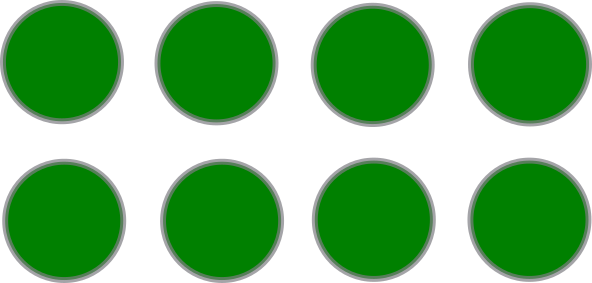
\includegraphics[width=.5\linewidth]{entropy_cluster/step1.png}
			\caption{Free particles. $H=3$}
		\end{subfigure}
		\begin{subfigure}{.5\textwidth}
			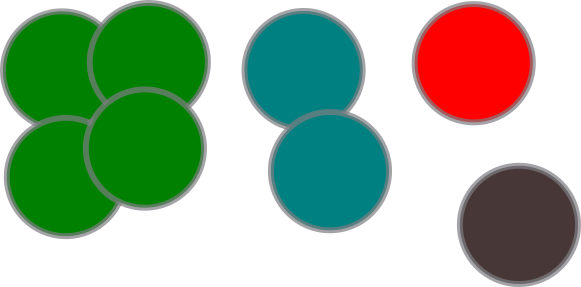
\includegraphics[width=.5\linewidth]{entropy_cluster/step2.png}
			\caption{Some Free and Some Bound Particles.\\ $0 < H < 3$}
		\end{subfigure}
		\begin{subfigure}{.5\textwidth}
			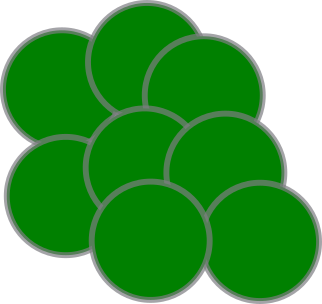
\includegraphics[width=.5\linewidth]{entropy_cluster/step3.png}
			\caption{Bount particles. $H=0$}
		\end{subfigure}
		\caption{entropy of a system of $8$ particles}
	\end{figure}
	

	\subsection{Specific Heat, $C(p,L)$}
	\label{subsect.percolation.specific-heat}
	According to the definition of specific heat in thermodynamics (\ref{def:specific-heat-thermodynamics})  we can find specific heat if we know the temperature and entropy. In percolation theory we measure the Shannon entropy, $H(p,L)$. And we use $(1-p)$ as the analogue of temperature which gives
	\begin{align}
		C &= (1-p) \frac{dH}{d(1-p)} \\
		  &= -(1-p) \frac{dH}{dp}
		  \label{def:specific-heat-percolation}
	\end{align}
	using this definition we can easily find the specific heat of the percolating system. And from specific heat we obtain the critical exponent $\alpha$ from the scaling relation in section (\ref{subsect:list-of-exponents}) which turns out to be
	\begin{equation}
		C = L^{\alpha/\nu} \phi_C(\left(p-p_c\right)L^{1/\nu})
	\end{equation}
	Here we have used FSS hypothesis (\ref{sect:fss}).
	Therefore plotting $C L^{-\alpha/\nu}$ vs $\left(p-p_c\right)L^{1/\nu}$ would give us a data collapse.
			
	
	\subsection{Order Parameter, $P(p,L)$}
		From above discussion we can say that if $p\geq p_c$ the spanning cluster exists but we still cannot say if a randomly chosen site belongs to the spanning cluster. Therefore we need to quantify the strength of the spanning cluster. Percolation strength or $P$ is defined as the probability to find the site that belongs to the spanning cluster, meaning randomly pick a site and what is the probability that the selected site will belong to the spanning cluster. And this quantity should depend on occupation probability $p$ and system size $L$. We call it Percolation Strength or sometimes Order Parameter as it describes the measure of order in the system. Order means the likeliness of not getting confused. If all clusters of same size, i.e. identical, we will get confused which cluster we have chosen ($p=0$ case) but if there is only one cluster there is no chance of confusion ($p=1$ case).\\
		We define the percolation strength as
		\begin{equation}
			P = \frac{\text{number of sites in the spanning cluster}}{\text{total number of sites in the lattice}}
		\end{equation}
		But in a system where there are no boundary, e.g. a network or Bethe lattice, the idea of spanning cluster is not valid. Then we use the largest cluster to define the percolation strength
		\begin{equation}
			P = \frac{\text{number of nodes in the largest cluster}}{\text{total number of nodes in the network}}
		\end{equation}
		Both definition, though looks a bit different when plotted, gives the same critical exponent $\beta$. How to find this exponent is shown in section (\ref{subsect:order-parameter}).
		
	    Mathematically
		\begin{align}
			P(p,L) &= \frac{K}{\sum_{i} k_i}
			\label{def:order-parameter}
		\end{align}
		where $K$ is the size of the spanning cluster and $k_i$ is the size of the $i-th$ cluster.
		Percolation strength is the Order parameter of the system which is the measure of Order of a system.
		Note that, with periodic boundary condition we have
		\begin{equation}
			\sum_{i} k_i = L^2
		\end{equation}
		and without periodic boundary condition
		\begin{equation}
			\sum_{i} k_i = L(L-1)
		\end{equation}
		
		Order parameter is related to the exponent $\beta$		from the scaling relation in section (\ref{subsect:list-of-exponents}) which turns out to be
		\begin{equation}
		P = L^{-\beta/\nu} \phi_P(\left(p-p_c\right)L^{1/\nu})
		\end{equation}
		Here we have used FSS hypothesis (\ref{sect:fss}).
		Therefore plotting $P L^{\beta/\nu}$ vs $\left(p-p_c\right)L^{1/\nu}$ would give us a data collapse.
			 
			 
	\subsection{Susceptibility, $\chi(p,L)$}
		In percolation we measure susceptibility using jumps of the size of the largest cluster, i.e., $\Delta P$. We keep track of the size of the largest cluster for each change of $p$, i.e. $\Delta p$. Then the jump per unit change of $p$ tells us what the susceptibility is. Mathematically
		\begin{equation}
			\chi = \frac{\Delta P}{\Delta p}
		\end{equation}
		for a lattice of length $L$ there are $L^2$ sites and occupying one site increase $p$ by $1/L^2$ therefore for site percolation $\Delta p = 1 /L^2$ and for bond percolation it is $\Delta p = 1 / 2 L^2$.		Susceptibility can also be measured by differentiating the order parameter $P$ with respect to $p$ and it would give the same exponent upon measurement.
		
		
		Susceptibility is related to the exponent $\gamma$		from the scaling relation in section (\ref{subsect:list-of-exponents}) which turns out to be
		\begin{equation}
		\chi = L^{\gamma/\nu} \phi_\chi(\left(p-p_c\right)L^{1/\nu})
		\end{equation}
		Here we have used FSS hypothesis (\ref{sect:fss}).
		 Therefore plotting $\chi L^{-\gamma/\nu}$ vs $\left(p-p_c\right)L^{1/\nu}$ would give us a data collapse.
		 

	\subsection{Fractal Dimension, $d_f$} 
		\label{subsect:fractal-dim}
		 A fractal \cite{Falconer2003} is an object which occupies less space than it is embedded. For example a piece of cheese is a 3D fractal, since there are holes in the cheese which is empty. The spanning cluster shows a behaviour to be a fractal.		The spanning cluster is a unique cluster that spans the entire lattice (or wraps around the lattice). But the size of the spanning cluster varies with the size of the lattice and it is related as
		\begin{equation}
			S \sim L^{-d_f}
		\end{equation}
		here $S$ is the size of the spanning cluster and $d_f$ is known as the fractal dimension. If we plot $\log S$ vs $\log L$ we will find a straight line with negative slope which has value $d_f$. Thus $d_f$ gives us the size of spanning cluster for a lattice of length $L$.
	
	\subsection{Cluster Size Distribution Function, $n_s$} \label{subsect:cluster-size-dist-func}
		At the critical point there exists many clusters of different sizes. Say we have $m$ distinct cluster meaning none of the $m$ clusters are of same size. $n_1, n_2, \ldots, n_m$ is the number of times cluster of size $1, 2, \ldots, m$ appears divided by the total number of cluster. Therefore we will have
		\begin{equation}
			\sum_{s} n_s s = 1
		\end{equation}
		where $s$ is the size of a cluster and $n_s$ is the frequency of the occurrence of the cluster of size $s$. They seem to follow the power law
		\begin{equation}
		n_s(p_c)\sim s^{-\tau}
		\end{equation}
		Thus if we know the size of the cluster at $p_c$ we can tell approximately the number of time that cluster appears and vice versa.
	

\section{Exact Solutions}
	Percolation problem can be solved exactly in $1$ and $\infty$ dimension. In dimension $1 < d < \infty$ there is not analytical solution, it can only be solved approximately using simulations. Analytic solution in dimension greater than $1$ and less than $\infty$ is a still to be solved problem. Interestingly, many of the features found in one dimension seem to be valid for higher dimensions too. Thus using the insight of these exact solutions in $1$ and $\infty$ dimension we get a window into the world of phase transitions, scaling and critical exponents.
	\subsection{One Dimension}
		\subsubsection{Threshold}
		The simplest lattice one can think of is the one dimensional lattice. It consists of many sites arranged at an equidistant positions along a line. Each site of the lattice can either be occupied with probability $p$ or remain empty with probability $1-p$. Thus there are only two possible states of each site.
		\begin{figure}
			\includegraphics[width=\linewidth]{{{1d_lattice}}}
			\caption{One Dimensional Lattice. Empty ones are white and filled ones are black.}
			\label{fig:1d-lattice}
		\end{figure}
		A cluster is a group of neighboring occupied sites which contains no empty sites in between. A single empty sites splits a cluster into two clusters. If we find $n$ successive occupied sites, we say that it forms a cluster of size $n$. We want to find the probability at which an infinite cluster appears for the first time, i.e., the critical occupation probability.\\
		Let $\omega(p,L)$ is the probability that a linear chain of size $L$ has percolating cluster at probability $p$. Note that, if two sites form one cluster, the probability that we find such cluster is $p^2$. Similarly if we want a cluster containing $L$ sites the probability is $\omega(p,L) = p^L$, means $L$ successive sites are occupied independent of each other. 
		\begin{equation}
			\lim_{L \rightarrow \infty} omega(p,L) = 
			\begin{cases}
			  0 \text{ , } \forall p < 1
			  \\
			  1 \text{only if p = 1}
			\end{cases}
		\end{equation}
		For $p=1$ all sites of the lattice are occupied and a percolating cluster spans from $-\infty$ to $\infty$ so that each and every and every sites of the lattice belong to the percolating cluster.For $p<1$ we will have on the average $(1-p)^L$ empty sites. So if $L \rightarrow \infty$, we have $(1-p)^L \rightarrow const.$ revealing that there will be at least one, if not more, empty site somewhere in the chain. Which proves that as long as $p<1$ there is no spanning cluster. Thus the percolation threshold or the critical occupation probability in one dimension is
		\begin{equation}
			p_c = 1
		\end{equation}
		\subsubsection{Cluster Size}
		A cluster of size $s$,a.k.a. $s$-cluster, is formed when $s$ successive sites are occupied and they are surrounded by two empty sites. Probability of $s$ successive sites are being occupied is $p^s$ and $2$ sites are unoccupied is $(1-p)^2$. Thus the probability of picking a cluster at random that belongs to an $s$-cluster is
		\begin{equation}
			n_s = p^s (1-p)^s
			\label{eqn:n_s-1d}
		\end{equation}
		$n_s$ is also the number of $s$-clusters per lattice site. Note that the state of one particular site is independent of any other sites, that's why we multiply probabilities. Further manipulation of equation (\ref{eqn:n_s-1d}) gives
		\begin{equation}
			n_s = (1-p)^2 \exp (s \ln p) = (1-p)^2 \exp(-s/\xi)
		\end{equation}
		where $\xi$ is the correlation length and defined as
		\begin{equation}
			\xi = -\frac{1}{\ln p} = - \frac{1}{\ln(p_c - (p_c -p))} \sim (p-p_c)^{-1} = (p-p_c)^\nu
			\label{eqn:correlation-length-def}
		\end{equation}
		in the limit $p\rightarrow p_c$ and since $p_c=1$.
		\subsubsection{Mean Cluster Size}
		The probability that an arbitrary site is in $s$-cluster is larger by a factor of s. This site can be any of the sites in the $s$-cluster. The probability that an arbitrary chosen site belongs to a cluster of size $s$ is $n_s s$, since $n_s$ is known to be the number of $s$-clusters per lattice site. Every occupied site must belong to one cluster even if it is a cluster of only one site, i.e., a cluster of size unity.  The probability that an arbitrary site belongs to a cluster is therefore proportional to the probably
		$p$ that it is occupied.
		\begin{equation}
			\sum_{s=1}^{\infty} s n_s = \frac{\text{number of total occupied sites}}{\text{number of total lattice sites}} = p
			\label{eqn:occupation-probability-in-mean-cluster-size}
		\end{equation}
		A quick check of the validity of equation (\ref{eqn:occupation-probability-in-mean-cluster-size}) can be performed using equation (\ref{eqn:n_s-1d}).
		\begin{align}
			\sum_{s=1}^{\infty}	s n_s \nonumber
			&=  \sum_{s} s (1-p)^2 p^s \nonumber \\
			&= (1-p)^2 \sum_{s} s p^s  \nonumber \\
			&= (1-p)^2 \sum_{s} p \frac{d(p^s)}{dp} \nonumber \\
			&= (1-p)^2 p \frac{d \sum_{s} p^s}{dp} \nonumber \\
			&= (1-p)^2 p \frac{d p(1-p)^{-1}}{dp} \nonumber \\
			&= (1-p)^2 p \left(\frac{1}{1-p} + \frac{p}{(1-p)^2}\right) \nonumber \\
			&= p 
		\end{align}
		Here we have used the series sum (\ref{eqn:series-sum-1}).
		\begin{align}
			\sum_s p^s 
			&= p + p^2 + p^3 + \ldots \nonumber \\
			&= p( 1 + p + p^2 + \ldots) \nonumber \\
			&= p(1-p)^{-1}
			\label{eqn:series-sum-1}
		\end{align}
		An important question one can ask is that what is average size of the cluster that we are hitting. Since $n_s s$ is the probability that an arbitrary site belongs to an $s$-cluster and $\sum_{s} n_s s$ is the probability that it belongs to any cluster. Thus we define $w_s$ as
		\begin{equation}
			w_s = \frac{n_s s}{\sum_{s} n_s s}
			\label{eqn:arbitrary-cluster-exactly-s-sites}
		\end{equation}
		$w_s$ is the probability that the cluster to which an arbitrary occupied site belongs contain exactly $s$ sites. The average cluster size $S$ is therefore
		\begin{eqnarray}
			S = \sum_{s} w_s s
		\end{eqnarray}
		This equation is very much similar to
		\begin{equation}
			\bar{x} = \int x p(x) dx
		\end{equation}
		using equation (\ref{eqn:arbitrary-cluster-exactly-s-sites}) we get
		\begin{align}
			S 
			&= \frac{\sum_{s} n_s s^2}{\sum_{s} n_s s} \nonumber \\
			&= \sum_{s=1}^{\infty} \frac{s^2 n_s}{p} \nonumber\\
			&= \frac{(1-p)^2}{p} \sum_{s=1}^{\infty} s^2 p^s \nonumber \\
			&= \frac{(1-p)^2}{p} \left(p \frac{d}{dp}\right)^2 \left(\sum_{s=1}^{\infty} p^s\right) \nonumber \\
			&= \frac{(1-p)^2}{p} \left(p \frac{d}{dp}\right)^2 (p(1-p)^{-1}) \nonumber \\
			&= p(1-p)^2 \frac{d^2}{dp^2} (p(1-p)^{-1}) \nonumber \\
			&= p(1-p)^2 \frac{d}{dp}(1-p)^{-2} \nonumber \\
			&= p(1-p)^2 2 (1-p)^{-3} \nonumber \\
			&= \frac{2p}{1-p} \nonumber \\
			&= \frac{1 + p}{1 - p}
		\end{align}
		we can write
		\begin{equation}
			S(p) = \frac{1-p}{1 + p} = \frac{p_c + p}{p_c - p}
		\end{equation}
		using the fact that $p_c = 1$ in 1D lattice.
		This equation reveals that the mean cluster size diverges for $p\rightarrow p_c$ where the minus	sign signifies that we are approaching from below $p_c$. This is in sharp contrast with	higher dimensional ones where we can approach to $p_c$ from either end while in one	dimension we cannot have access to the state $p > p_c$ . We thus find the mean cluster	size diverges following power law as we have \cite{nesm-lecture-notes}
		\begin{equation}
			S(p) \sim (p_c - p)^{-1}
		\end{equation}
		We encounter the similar behaviour in the higher dimensions also.
		
		\subsubsection{Correlation Function and Correlation Length}
		The correlation function or pair connectivity $g(r)$ is the probability that a site at position $r$ from an occupied site belongs to the same finite cluster. We are not including the contribution of the infinite cluster. This is valid infinite cluster does not exists as long as $p<1$. Let $r=0$ then $g(r=0)=1$ since the site at $r=0$ is the selected occupied site by definition. For 1D case a site at $r$ to be occupied and belongs to the same finite cluster, we will need $r$ subsequent sites and the probability of getting this is $p^r$. Therefore
		\begin{equation}
			g(r) = p^r
		\end{equation}
		It can also be expressed in terms of correlation length $\xi$
		\begin{equation}
			g(r) = \exp (\ln(p^r)) = \exp(-r/\xi)
		\end{equation}
		where $\xi$ is the correlation length (\ref{eqn:correlation-length-def}).\\
		Now that we have correlation function, we can define mean cluster size in terms of it
		\begin{equation}
			S = 1 + \sum_{r=1}^{\infty} g(r)
			\label{eqn:mean-cluster-size-correlation-function}
		\end{equation}
		At this point it is evident that the cutoff cluster size $s_\xi$ , mean cluster size $S(p)$, and correlation length $\xi$ diverges at the percolation threshold. The divergence has the form of a	simple power law of the distance from the critical occupation probability. In higher dimensional percolation problem this observation is also valid.
		
	\subsection{Infinite Dimension}
	Apart from one dimension percolation problem can be solved in infinite dimension. For this we need a suitable playground such as Bethe lattice. Bethe lattice lattice is a special type of lattice  where each site has $z$ neighbors and each branch gives rise to $(z-1)$ other branches. Figure (\ref{fig:bethe-lattice}) shows the Bethe lattice for $z=3$. Note that for $z=2$ we have nothing but the one dimensional lattice. \subsubsection{Properties of infinite dimensional object}
	For a 3D object the surface area is has dimension to $L^2$ and volume as dimension $L^3$. The same pattern is true of object in any dimension. If we denote area by $A$ and volume by $V$ for any dimension we have
	\begin{equation}
		A \propto V^{1-1/d}
	\end{equation}
	now as $d \rightarrow \infty$ we have
	\begin{equation}
		A \propto V
	\end{equation}
	Therefore if we find that the area of any object is proportional to its volume we can say it is an infinite dimensional object.
	\subsubsection{Bethe Lattice}
	In order to construct Bethe lattice for any $z$ we start with a central point which will be connected to $z$ sites. For example if $z=3$ then we will have a central site connected to $3$ sites by a branch and when we go to next layer each branch will be divided to $2$ more branches and this process will be continued up to $r$ layers (\ref{fig:bethe-lattice}). Only at the surface of the lattice, where the branching is stopped, is only one bond or branch connecting the surface site to the interior. There is only open loops in this structure, which means	that if we never change direction always reach new site if we never go back.Number of sites in the Bethe lattice increases exponentially with the distance from the origin, whereas in any $d$-dimensional lattice structure it	would increase with distance $d$ . In the case of Bethe lattice with $z=3$, the origin is surrounded by a shell of three sites ("first generation"), in the second shell we have six sites followed by a third	generation of twelve sites, etc.
	\begin{figure}
		\centering
		\includegraphics[width=10cm]{{{bethe-lattice}}}
		\caption{Bethe Lattice for $z=3$}
		\label{fig:bethe-lattice}
	\end{figure}
	After $r$ generation the total number of sites in the Bethe lattice is
	\begin{equation}
		1+3\times(1 + 2 + \ldots + 2^{r-1}) = 3.2^r - 2
	\end{equation}
	The number $3\times 2^{r-1}$ is the number of sites at the surface.
	Here we have used the following finite series sum
	\begin{equation}
		1+2+2^2+2^3+\ldots+2^r = 2^{r+1} - 1
	\end{equation}
	And if we measure the surface to volume ratio we get
	\begin{equation}
		\frac{A}{V} = \frac{number of sites in the surface}{total number of sites} = \frac{3\times 2^{r-1}}{3\times2^r - 2}
	\end{equation}
	as $r\rightarrow\infty$ we get
	\begin{equation}
		\frac{A}{V} \sim \frac{3\times 2^{r-1}}{3\times2^r} = \frac{1}{2} = constant
	\end{equation}
	Therefore Bethe lattice is indeed an infinite dimensional lattice.
	\subsubsection{Percolation Threshold}
	Percolation threshold of Bethe lattice is the occupation probability at which an infinite cluster appears for the first time. To find it we start walking from the origin and after one step we have $z-1$ new bonds that is connected to $z-1$ new sites in those direction. On the average there will be $(z-1)p$ occupied sites. And for each site there will be another $z-1$ branch and those bonds are connected to $(z-1)p$ sites on the average and so on. After $r$ step we will have an infinite cluster at probability $((z-1)p)^r$. Since $r\rightarrow \infty$ we have $((z-1)p)^r = 0$ if $(z-1)p < 1$. Thus we choose $(z-1)p = 1$ so that we will get an infinite cluster. That lead us to the desired critical  occupation  probability
	\begin{align}
		(z-1)p_c &= 1 \nonumber \\
		p_c 	 &= \frac{1}{z-1}
	\end{align}
	For $z=3$ we have $p_c = 1/2$.
	\subsubsection{Percolation Strength}
	Percolation strength of an infinite cluster is the probability of any arbitrary site to be the part of the infinite cluster. For the sake of calculation, for $p>p_c$ in the Bethe lattice, we introduce a new quantity $Q$ as the probability that an arbitrary site is note connected to the infinite cluster through a fixed branch originating from this site. Restricting ourselves to the lattice with $z=3$ and using basic probability theory, the strength 
	\begin{equation}
		P(p) = p(1-Q^3)
	\end{equation}
	Here $p$ is the probability that the site is occupied and $(1-Q^3)$ is the probability that at least one branch is connected to infinity.\\
	The probability that the two subbranches which start at the neighbor are not both leading infinity is	$Q^2$. The quantity $pQ^2$ is the probability that this neighbor is occupied but not connected to infinity	by any of its two subbranches. This neighbor is empty with probability $(1-p)$, in which case even	well connected subbranches do not help it. This gives us,
	\begin{equation}
		Q = (1-p) + p Q^2
	\end{equation}
	This is the probability that this fixed branch does not lead to infinity, either because the connection	is already broken at the first neighbor, or because later something is missing in the subbranch. So the solution of this quadratic equation is
	\begin{equation}
		Q = 1, \frac{1-p}{p}
	\end{equation}
	For $z$ neighbors, in general we have
	\begin{equation}
		Q = 1, 1 - \frac{2p(z-1)-2}{p(z-1)(z-2)}
	\end{equation}
	for $p<p_c$, there are no infinite clusters, fo with probability $1$ there are no connection to infinity. Now we use Taylor expansion for $P(p)$ around $p=p_c=1/2$
	\begin{align}
		P(p) = 
		\begin{cases}
		0	&\text{ for } p < p_c \\
		p\left(1- \left(\frac{1-p}{p}\right)^3\right) &\text{ for } p \geq p_c
		\end{cases}
	\end{align}
	Let,
	\begin{equation}
		f(p) = \left(\frac{(1-p)}{p} \right)^3
	\end{equation}
	Then
	\begin{align}
		f^\prime(p) &= -3p^-4 (1-p)^3 - 3 p^-3 (1-p)^2 \nonumber \\
		&= -\frac{3}{p} \left(\frac{(1-p)}{p}\right)^3 -\frac{3}{p} \left(\frac{(1-p)}{p}\right)^2
	\end{align}
	\begin{align}
		P(p) &= P(p_c) + (p-p_c) P^\prime(p_c) + \ldots \\
		&= 0 + (p-p_c) \left(1-f(p_c) - p f^\prime(p_c)\right) + \ldots \\
		&= 6(p-p_c) + \ldots \\
	\end{align}
	Therefore we get
	\begin{equation}
		P(p) \propto (p-p_c) \ \text{for} p \rightarrow p_c^+
	\end{equation}
	the critical exponent $\beta$ is defined by
	\begin{equation}
	P(p) \propto (p-p_c)^\beta
	\end{equation}
	Thus in Bethe lattice $\beta = 1$.
	\subsubsection{Mean Cluster Size}
	In case of Bethe lattice the mean cluster size is defined as the average number of sites to which the origin belongs. Let $T$ be the mean cluster size for one branch, that is the average number of sites to which the origin is connected and which belongs to one branch. Again, subbranches have the same mean cluster $T$ as the branch itself. If the neighbor is empty the cluster size for this branch is zero. If the neighbor is occupied, it contributes its own mass to the cluster which is unity and adds the mass $T$ for each of its two subbranches. Thus,
	\begin{equation}
		T = (1-p) \times 0 + p(1+2T)
	\end{equation}
	Solving this we get
	\begin{equation}
		T = \frac{p}{1 - 2p}
	\end{equation}
	for $p<p_c$. \\
	The total cluster size is zero if the origin is empty and $(1+3T)$ if the origin is occupied. Therefore the mean cluster size $S(p)$ is
	\begin{align}
		S(p) &= 1 + 3 T \\
		     &= \frac{1+p}{1-2p} \nonumber\\
   		     &= \frac{1+p}{2(p_c-p} \nonumber \\
   		     &=\frac{1+p}{2} (p_c - p)^{-1}
	\end{align}
	Thus the critical exponent $\gamma = 1$ for Bethe lattice. This is the exact result for mean cluster size and we notice that it diverges for $p\rightarrow p_c$.
	\subsubsection{Correlation Function and Correlation Length}
	The radial correlation function $g(r)$ is the average number of occupied sites within the same cluster at a distance $r$ from an arbitrary occupied site. The probability that a site at distance $r$ from the origin is occupied and the sites in between are occupied too is equal to $p^r$. Now if we think about a shell of radius $r$ then the number of all the sites enclosed by this shell is $z(z-1)^{r-1}$. Thus
	\begin{align}
		g(r) &= z(z-1)^{r-1} p^r \\
			 &= \frac{z}{z-1} \left(p(z-1)\right)^r \\
			 &= \frac{z}{z-1} \exp \left[\log\left[p(z-1)\right]\right]
	\end{align}
	The value of percolation threshold for Bethe lattice can be found by analyzing the behaviour of the correlation function at large distances, i.e. at r $\rightarrow \infty$. For $p(z-1) < 1$, $g(r)$ decreases exponentially, on the other hand for $p(z-1)>1$, the correlation function diverges which signifies the existence of an infinite cluster. Mathematical treatment yields the correlation length from (\ref{eqn:correlation-length-def})
	\begin{align}
		\xi &= \frac{-1}{\log[p(1-z)]} \nonumber \\
			&= \frac{-1}{\log(p/p_c)} \nonumber \\
			&= (p-p_c)^{-1}
	\end{align}
	as $p$ approaches $p_c$, that is $\nu = 1$. \\
	Clearly the 1D lattice and Bethe  lattice exhibits power law while we approach a critical value which suggests the same phenomena in other variants of such problems.

\section{Algorithm} \label{sect:algorithm}
	In the classical Hosen-Kopelman algorithm for percolation model \cite{Hoshen1976}, one first choose an occupation probability $p$ and then generate a number $r$ for each site of the lattice. The site is occupied if $r \leq p$ and remain empty if $r > p$. One therefore create an entire new state of a given lattice size for every different value of $p$. Note that the number of occupied sites $n$ for a given $p$ may very in each realization. However, the expected or ensemble average over $M$ experiments will give $n = p M$ in the limit $M \rightarrow$. Thus the number of occupied bonds or sites is also a measure of $p$. Using this idea Ziff and Newman \cite{Newman2001} proposed an algorithm which generate states for each value of $n$ from zero up to some maximum value $n = L^2$ for site percolation on $L\times L$ square lattice for instance. In this way, one can save some effort by noticing the fact that a new state with $n + 1$ occupied sites or bonds can be created by adding one extra randomly chosen site or bond to the state containing n sites or bonds. The first step of their algorithm is to decide an order in which the bonds or sites are to be occupied. That is, every attempt to occupy a bond/site is successful.
	
	\subsection{Square Lattice}
	A square lattice is an ideal playground for percolation. 	A square lattice of linear size $L$ has 
	$L^2$ sites connected by $2L^2$  bonds with periodic boundary condition and by
	$2L(L-1)$ bonds without periodic boundary condition. All sites are equally separated from each other at a certain distance. And all sites have exactly four neighbor. Since with the periodic boundary condition the sites in the left edge are connected with the sites in the right edge and same rule for sites in the top and bottom edges. We always want our experimental result in the thermodynamic limit. This means that we want the results for a lattice where $L\rightarrow \infty$. In other words the sites are densely spaced. But that is practically impossible. The simple solution to this problem is to use number of large lengths, (say $L = \{L_1, L_2, \ldots L_n \}$, where $n$ is a finite number and $L_1 < L_2 < \ldots < L_n$), and extrapolate the results for infinite lattice. The visual structure of the square lattice is as follows (\ref{fig:sq_lattiec_empty}). This is and empty lattice structure. Filled circles are for occupied site and filled bonds are for occupied bonds (\ref{fig:site_bond_symbol}).
	
	\begin{figure}[htbp]
		\centering
		\begin{subfigure}{.8\textwidth}
			\centering
			\includegraphics{{{square-lattice-5x5_skeleton}}}
			\caption{}
			\label{fig:sq_lattiec_empty}
		\end{subfigure}
		\begin{subfigure}{.2\textwidth}
			\centering
			\includegraphics[width=.1\linewidth]{{{site_empty}}}
			\caption{}
		\end{subfigure}
		\begin{subfigure}{.2\textwidth}
			\centering
			\includegraphics[width=0.1\linewidth]{{{site_occupied}}}
			\caption{}
		\end{subfigure}
		\begin{subfigure}{.2\textwidth}
			\centering
			\includegraphics[width=.1\linewidth]{{{bond_empty}}}
			\caption{}
		\end{subfigure}
		\begin{subfigure}{.2\textwidth}
			\centering
			\includegraphics[width=.1\linewidth]{{{bond_occupied}}}
			\caption{}
		\end{subfigure}
		\caption{ (a) Square Lattice (empty skeleton) of length $L=5$ where all sites and bonds are empty(b) Empty site (c) Occupied site (d) Empty bond (e) Occupied bond.}
		\label{fig:site_bond_symbol}
	\end{figure}
	Percolation 
	is known as site or bond type depending on whether we occupy sites or bonds respectively. Here we describe bond percolation process in detail and site percolation in brief.

	\subsection{Bond Percolation}
		\label{bond-percolation}
		One of the famous percolation type is random bond percolation on square lattice. Here we assume that all the labeled
		bonds are initially frozen. The rule  is then  to choose 
		one frozen bond at each step randomly with uniform probability and occupy it. We continue the process one by one till the 
		occupation probability $p$, fraction of the total bonds being occupied, reaches to unity. 
		At $p=0$ each site is a cluster of its own size and as $p$ is tuned towards increasing $p$
		then we observe clusters, a group of sites connected by occupied bonds, are continuously
		formed and grown on the average. In the process there 
		comes a critical state when occupation of just one more bond results in the emergence of a 
		cluster that spans 
		across the entire system for the first time. This process of cluster growth is shown in figure (\ref{fig:cluster-growth-bond}).
		\begin{figure}[h]
			\centering
			\captionsetup[subfigure]{width=0.9\textwidth}
			\begin{subfigure}[t]{0.325\textwidth}
				\centering
				\includegraphics[width=0.95\linewidth]{{{bond-square-lattice-5x5_step0}}}
				\caption{Initial state of a square lattice of linear length $L=5$. Total $5^2$ sites and $2\times 5^2$ frozen bonds.}
			\end{subfigure}
			\begin{subfigure}[t]{0.325\textwidth}
				\centering
				\includegraphics[width=0.95\linewidth]{{{bond-square-lattice-5x5_step1}}}
				\caption{One bond is occupied and it connects two cluster of size one to create one cluster of size two.}
			\end{subfigure}
			\begin{subfigure}[t]{0.325\textwidth}
				\centering
				\includegraphics[width=0.95\linewidth]{{{bond-square-lattice-5x5_step2}}}
				\caption{Another bond is occupied and it connect two cluster of size two and one to create one cluster of size three.}
			\end{subfigure}
			\caption{Cluster growth in bond percolation in initial state.}
			\label{fig:cluster-growth-bond}
		\end{figure}
		Notice that if occupying a bond can be of two kind. one is intercluster connection where two distinct cluster is connected to form a larger cluster whose size is the sum of the connecting cluster. Another is the intracluster connection where two end of same cluster is connected but the cluster size remains invariant. Figure (\ref{fig:cluster-growth-bond-inter-intra}) demonstrate this process.
		
		\begin{figure}[h]
			\centering
			\captionsetup[subfigure]{width=0.9\textwidth}
			\begin{subfigure}[t]{0.325\textwidth}
				\centering
				\includegraphics[width=0.95\linewidth]{{{bond-square-lattice-5x5_cluster-1}}}
				\caption{Two cluster is present. Red one has size  $5$ and green one has size $3$.}
			\end{subfigure}
			\begin{subfigure}[t]{0.325\textwidth}
				\centering
				\includegraphics[width=0.95\linewidth]{{{bond-square-lattice-5x5_cluster-2}}}
				\caption{Intracluster connection results in only increase of the occupation probability. Cluster size remains the same.}
			\end{subfigure}
			\begin{subfigure}[t]{0.325\textwidth}
				\centering
				\includegraphics[width=0.95\linewidth]{{{bond-square-lattice-5x5_cluster-3}}}
				\caption{Intercluster connection. Red cluster of size $5$ and green cluster of  size $3$ merges to form a new cluster (red) of size $8$. }
			\end{subfigure}
			\caption{Intercluster and intracluster connection.}
			\label{fig:cluster-growth-bond-inter-intra}
		\end{figure}
		
		Using this process in mind we measure various quantity, for example Entropy, Spanning probability, Order Parameter etc., and the we use the scaling relation to obtain the exponents which is done in chapter (\ref{chapter:ballistic-deposition}) for site percolation.
		
		
		
	\subsection{Site Percolation}
		Here we discuss the traditional definition of site percolation and in section (\ref{sect.redefinition-site-percolation}) we discuss what goes wrong if we use this definition and how we can resolve them in detail which is one of the purpose of this thesis.
		
		Now in site percolation we take a square lattice of linear length $L$ which have $L^2$ sites. We occupy each site with probability $p$ and keep it empty with probability $(1-p)$. Thus after we have visited all the sites in the lattice we get to measure any quantity of this system for probability $p$. Here we measure the cluster size by number of sites in the cluster as we do in bond percolation. In this way we get to measure a quantity for a fixed probability $p$ in each realization which is the classical Hoshen-Koppelman (HK) algorithm \cite{Hoshen1976}. 
		
		Instead we we Newman-ziff algorithm so that we can measure various observable quantities over the entire range of $p$ in every 
		realization instead of measuring them for a fixed probability $p$ in each realization \cite{Newman2001}. In NZ algorithm we pick a site at random with uniform probability and occupy it. Thus if we occupy $n$ sites we get a system with occupation probability $p=n/N$ where $N=L^2$. This process is further discussed in the next section (\ref{subsect.nz-algrithm}).
	
	\subsection{Newman-Ziff (NZ) algorithm}	
		\label{subsect.nz-algrithm}
		To study random percolation, we use Newman-Ziff (NZ) algorithm as 
		it helps calculating various observable quantities over the entire range of $p$ in every 
		realization instead of measuring them for a fixed probability $p$ in each realization \cite{Newman2001}.
		On the other hand, in classical Hoshen-Koppelman (HK) we can only measure an observable quantity
		for a given $p$ in every realization and this is why NZ is more efficient than HK \cite{Hoshen1976}.
		To illustrate the idea we consider the case of bond percolation first. 
		According to the NZ algorithm, all the labelled bonds $i=1,2,3,..., M$ 
		are first randomized and then arranged in an order 
		in which they will be occupied. Note that the number of bonds with periodic
		boundary condition is $M=2L^2$. In this way we 
		can create percolation states consisting of $n+1$ occupied bonds
		simply by occupying one more bond to its immediate past state consisting of $n$ occupied 
		bonds. Initially, there are $N=L^2$ clusters of size one.
		Occupying the first bond  means forming a cluster of size two (four). However, 
		as we keep occupying thereafter, average or mean cluster size keep growing 
		at the expense of decreasing cluster number. Interestingly, all the observables in percolation, this
		way or another, related to cluster size and hence proper definition of cluster is crucial.
		One of the advantages of the NZ algorithm is that we calculate an observable, say $X_n$, as 
		a function of the number of occupied bonds (sites) $n$ and use the resulting data in the convolution relation
		\begin{equation}
		\label{eq:convolution}
		X(p)=\sum_{n=1}^N p^n(1-p)^{N-n} X_n,
		\end{equation}
		to obtain $X(p)$ for any value of $p$. 
		The appropriate weight factor for each $n$ at a given $p$ is $\sum_{n=1}^N p^n(1-p)^{N-n}$ \cite{Newman2001}. 
		The convolution relation takes care of that weight factor and hence helps obtaining a smooth curve for $X(p)$.
		
		The detail discussion of the use of convolution relation and how we can efficiently implement in a program is discussed in Appendix (\ref{appendix.convolution}).



\section{Application}
\label{sect:application}
	Ever since the percolation phenomena was discovered it has been extensively used in wide range of science. Some of it is discussed here. Though limited, this discussion gives us the significance of percolation and enables us to appreciate it.
	\subsection{Epidemiology}
	Many diseases spread through human populations via close physical interactions. The interpersonal contact patterns that underlie disease transmission can naturally be thought to form a network, where links join individuals who interact with each other. During an outbreak, disease then spreads along these links. All epidemiological models make assumptions about the underlying	network of interactions, often without explicitly stating them.
	
	Percolation has long been an important tool in infectious disease epidemiology \cite{Bansal2007}. L Meyers gave a wonderful insight of contact	network epidemiology, a more powerful approach that applies bond percolation on random graphs	to model the spread of infectious disease through heterogeneous populations \cite{Meyers2006}.
	
	Before that	in 2000, Moore et al. studied some simple models of disease transmission on small-world networks \cite{Moore2000}. They showed that the resulting models display epidemic behavior when the infection	or transmission probability rises above the threshold for site or bond percolation on the network,	and they gave exact solutions for the position of this threshold in a variety of cases. 
	
	Alessandro	Vespignani and his team studied wifi networks and malware epidemiology. They developed an	epidemiological model that takes into consideration prevalent security flaws on these routers.They	simulated spread of such a contagion on real-world data for georeferenced wireless routers \cite{Hu2009}.
	
	Sander et al. considered a spatial model related to bond percolation for the spread of a disease that	includes variation in the susceptibility to infection. They worked on a lattice with random bond	strengths and showed that with strong heterogeneity, i.e. a wide range of variation of susceptibility, patchiness in the spread of the epidemic is very likely, and the criterion for epidemic outbreak	depends strongly on the heterogeneity. Their results were qualitatively different from those of standard models in epidemiology, but correspond to real effects \cite{Sander2002}.
	
	After the birth of scale free	network the study of epidemics has become even more popular among statistical physicists.
	
	
	\subsection{Neural Network and Cognitive Psychology}
	Percolation is used to understand the way activation and diffusion of neural activity occur within neural networks \cite{Friedenberg2011}. Iian Breskin's team in 2006 studied living neural networks by measuring the neurons' response to a global electrical stimulation. They showed through analysis that neural connectivity is lowered by reducing the synaptic strength, chemically blocking neurotransmitter receptors. They used a graph-theoretic approach to show that the connectivity undergoes a percolation transition. This occurs as the giant component disintegrates, characterized by a power law with an exponent $\beta \simeq 0.65$	 \cite{Breskin2006}.\\
	
	It is easiest to understand percolation theory by explaining its use in epidemiology \cite{Moore2000}. Individuals that are infected with a disease can spread it knowingly or unknowingly via social or physical interaction. It's easy to say that the more social a person is the more it is likely that he will spread more disease than the unsocial one. Therefore some factors, e.g., occupation, size of social circle etc, influence the rate of infection. \\
	
	
	Now, if one were to think of neurons as the individuals and synaptic connections as the social bonds between people, then one can determine how easily	messages between neurons will spread \cite{Friedenberg2011} When a neuron fires, the message is transmitted along	all synaptic connections to other neurons until it can no longer continue.
	
	 Synaptic connections are	considered either open or closed (like a social or unsocial person) and messages will flow along	any and all open connections until they can go no further. Just like occupation and sociability play	a key role in the spread of disease, so does the number of neurons, synaptic plasticity \cite{Hughes1958} and	long-term potentiation when talking about neural percolation. Percolating clusters are a single large	group of neurons that are all connected by open bonds and take up the majority of the network.	Any signals that originate at any point within the percolating cluster will have a great impact and	diffusion across the network than signals that original outside of the cluster.
	  This is much like	how a teacher is more likely to spread an infection to a whole community through contact with the	students and subsequently with the families than an isolated businessman that works from home.
	
	
	\subsection{Ferromagnetism}
	One of the most studied phase transition phenomena of physics is that para-magnetic to ferromagnetic transition. The magnetic spins of a magnetic material, e.g., nickel, interact with each other:	the energy is lower if the two spins on adjacent nickel atoms are parallel than if they are anti-parallel. This lower energy tends to cause the spins to be parallel and below a temperature called	the Curie temperature,$T_c$ , most of the spins in the nickel are parallel, their magnetic moments then	add up constructively and the piece of nickel has a net magnetic moment: it is a ferromagnetic.
	 Above the Curie temperature on average half the spins point in one direction and the other half in	the opposite direction. Then their magnetic moments cancels out, and the nickel has no net magnetic	moment. It is then a para-magnet. Thus at $T_c$ the nickel goes from having no magnetic moment to	having a magnetic moment. This is a sudden qualitative change and when this happens we say that	a phase transition has occurred. Here the phase transition occurs when the magnetic moment goes	from zero to non-zero. It is from the para-magnetic phase to the ferromagnetic phase.	So, this critical value $T_c$ of the temperature marking the borderline between the existence and	non-existence of so called spontaneous magnetization. A standard mathematical model for this	phenomenon is the Ising model \cite{Cipra1987}. It turns out that there are two parameters which specify	the conditional probabilities: the 'external magnetic field' $h$, and the strength $J$ of interaction	between neighbors. If $J = 0$, the states of different vertices are independent, and the process is	equivalent to site percolation \cite{Coniglio1976}. The relationship between the Ising model and bond percolation	is rather strong. It turns out that they are linked via a type of 'generalized percolation' called the other considerations \cite{Coleman1992, Seiden1990}. 
	 Studing the random-cluster model,
	 one can obtain conclusions valid simultaneously for percolation and the Ising model.
	 This discovery was made in 1970 by Fortuin and Kastelyn \cite{Fortuin1972a, Fortuin1972b, Fortuin1972c}, and it has
	 greatly influenced part of the current view of disordered physical systems
	 
	 
	\subsection{Cosmology}
	We know mass distribution and motions of the components of a galaxy are determined by gravity,	it has not been clear what is responsible for the striking morphology of a spiral galaxy such as	shown in the figure.
	\begin{figure}
		\centering
		\includegraphics[width=10cm]{{{galaxy}}}
		\caption{NGC $4414$, a typical spiral galaxy in the constellation Coma Berenices, is about $55,000$ light-years in diameter and approximately $60$ million light-years away from Earth.}
		\label{galaxy}
	\end{figure}
	 The spiral arms extend over 16,000 parsecs (1 parsecs equals 3.26 light-years), and the traditional view is that it is necessary to have a long-range interaction like gravity, which interacts with object that have mass,	to create such long-range order. However, in condensed matter physics it is well known that long-range order can be induced by a short-range interaction, and this is a characteristic feature of a	continuous phase transition [48].
	 
	The structural features of spiral galaxies arises from a percolation phase transition that underlies the phenomenon of propagating star formation. According to this	view, the appearance of spiral arms is a consequence of the differential rotation of the galaxy	and the characteristic divergence of correlation lengths for continuous phase transitions.
	
	 Other	structural properties of spiral galaxies, such as the distribution of the gaseous components and the	luminosity, arise directly from a feedback mechanism that pins the star formation rate close to the	critical point of the phase transition. At least for some galaxies, morphological and other features	are already fixed by general properties of phase transitions, irrespective of detailed dynamic or	other considerations \cite{Seiden1990, Coleman1992}.
	 
	 \subsection{Others}
	 Percolation model 
	 has also been applied to a wide variety of natural and social phenomena  such as the spread of
	 disease in a population \cite{Murray2007}, flow of fluid through porous media \cite{Dapp2016}, 
	 conductor-insulator composite materials \cite{McLachlan1990}, resilience of systems \cite{Barabasi2000, PastorSatorras2001}, 
	 dilute magnets  \cite{Bergqvist2004}, the formation of public opinion \cite{Watts2002, Shao2009, Morone2015}
	 and spread of biological and computer viruses leading to epidemic \cite{Newman1999, Moore2000}
	
	
	




		

		
	

	